\chapter{Literature Review}
\label{cha:Literature Review}

\section{Car Following Models}
\label{sec:Car Following Models}
\newtext{ALL SHOULD BE CONSIDERED NEW}

Most lane changing models stem from 'car-following models', which define actions for a vehicle based on the behaviour of its predecessors (the vehicles in front of it). One early car-following model was defined in 1981 by P.G. Gipps \citep{Gipps1981}. It was designed to mimic real-world driver behaviour, calculating a safe travel speed for a vehicle based on the speed of its predecessor. A safe travel speed is defined as a speed at which the driver can safely stop if the preceding driver stops.

Gipps' paper defines two equations, which provide constraints on the speed of vehicle $n$ at time $t + \tau$. $t$ is the current time and $\tau$ is the apparent reaction time, a constant for all vehicles. The first equation defines the acceleration constraint of the vehicle. It was obtained using measurements from an instrumented car.

\begin{equation}\label{Gipps1981Accel}
v_n(t+\tau) \leqslant v_n(t) + 2.5a_n\tau\Biggl(\frac{1 - v_n(t)}{V_n}\Biggr)\Biggl(\frac{0.025 + v_n(t)}{V_n}\Biggr)^{1/2}
\end{equation}

$v_n(t)$ is the speed of vehicle $n$ at time $t$. $a_n$ is the maximum acceleration the driver of vehicle $n$ wishes to undertake. $V_n$ is the target speed for vehicle $n$. The equation shows that the driver accelerates until close to their target speed. They then reduce their acceleration until it reaches zero. At this point the vehicle should be travelling at it's target speed.

The second constraint is the braking profile of the vehicle. This is given as

\begin{equation}\label{Gipps1981Brake}
\begin{split}
&v_n(t+\tau) \leqslant \\
&b_n\tau + \sqrt{\Biggl(b_n^2\tau^2 - b_n\biggl(2\Bigl[x_{n-1}(t) - s_{n-1} - x_n(t)\Bigr] - v_n(t)\tau - \frac{v_{n-1}(t)^2}{\hat{b}}\biggr)\Biggr)}
\end{split}
\end{equation}

$b_n$ is the most severe braking the driver of vehicle $n$ wishes to undertake. It is always a negative value, and should be considered negative acceleration. $\hat{b}$ is the driver of vehicle $n$'s best guess at $b_{n-1}$ where $n-1$ is $n$'s predecessor. $x_n(t)$ is the location of the front of vehicle $n$ at time $t$. $s_n$ is the effective size of vehicle $n$. This is equal to the physical length of $n$, plus a margin $n$'s successor is not willing to enter, even when $n$ is at rest. The equation shows that the  

Therefore, at time $t + \tau$, assuming the driver travels as fast as is safe, and within the limitations of the vehicle, the speed is given by the minimum of these two equations.

\begin{equation}
v_n(t) = \min{(\eqref{Gipps1981Accel},\eqref{Gipps1981Brake})}
\end{equation}

This model works well at describing the behaviour of traffic. However, translating this work to autonomous vehicles poses a number of problems. Firstly, the work is based on the behaviour of real-world drivers in instrumented vehicles. This introduces human driver variables into the equations. An autonomous vehicle with perfect sensors would have an almost negligible $\tau$, as the vehicles would have a very minimal reaction time. $s_n$ would also need to be adjusted. The margin added can be much less, as autonomous vehicles would be more precise than human drivers, driving closer to their predecessors. 

The model also ignores inter-vehicle communication. Autonomous vehicles could communicate their intentions to nearby vehicles, allowing them to act before they do. This could greatly reduce the following distance of successor vehicles, it would also allow vehicles to accelerate and move as a unit, or a 'platoon'. It would also allow autonomous vehicles to gain accurate value for $\hat{b}$.

In 2000 Treiber et al. suggested the 'Intelligent Driver Model' (IDM) \citep{Treiber2000}. This is the notation for the model

The acceleration of vehicle $\alpha$, $\dot{v_\alpha}$, is defined using a continuous function of its velocity, $v_\alpha$; the distance to the rear of its predecessor, $s_\alpha$; and the velocity difference of $\alpha$ and it's predecessor, also known as the approaching rate $\Delta v_\alpha$. The vehicle interactions are solely based on $\alpha$'s relative acceleration to its predecessor. The model only provides position information for a vehicle in relation to its predecessor, and it does not provide its velocity at a given time, as Gipps' model does. 

The IDM is broken into two components. The first describes the behaviour of a vehicle on a free road.

\begin{equation}
\dot{v_\alpha} = a^{(\alpha)}\Biggl[1 - \biggl(\frac{v_\alpha}{v_0^{(\alpha)}}\biggr)^\delta\Biggr]
\end{equation}

Here $a^{(\alpha)}$ is the maximum acceleration of vehicle $\alpha$ and $v_0^{\alpha}$ is the desired velocity of $\alpha$. $\delta$ is the acceleration exponent, which is typically 4. 

The second component describes the behaviour of a vehicle as it approaches its predecessor. 

\begin{equation}
\dot{v_\alpha} = - a^{(\alpha)}\biggl(\frac{s^*}{s_\alpha}\biggr)^2
\end{equation}

As the gap, $s_\alpha$, between $\alpha$ and it's predecessor, gets closer to the desired minimum gap $s^*$, $\alpha$ decelerates.

Interpolating the two components gives us the IDM. 

\begin{equation}
\dot{v_\alpha} = a^{\alpha}\Biggl[1 - \biggl(\frac{v_\alpha}{v_0^\alpha}\biggr)^\delta - \biggl(\frac{s^*(v_\alpha,\Delta v_\alpha)}{s_\alpha}\biggr)^2\Biggr]
\end{equation}

The desired minimum gap in the IDM varies dynamically with velocity and approaching rate. It is given by the following function.

\begin{equation}\label{IDMSpacingFunction}
s^*(v,\Delta v) = s_0^{(\alpha)} + s_1^{(\alpha)}\sqrt{\frac{v}{v_0^{(\alpha)}}} + T^\alpha v + \frac{v\Delta v}{2\sqrt{a^{(\alpha)}b^{(\alpha)}}}
\end{equation}

The equation takes the bumper-to-bumper space $s_0^{(\alpha)}$, also known as the minimum jam distance, and adds the comfortable jam distance $s_1^{(\alpha)}$. The bumper-to-bumper space is the minimum gap between $\alpha$ and its predecessor in stationary traffic. The comfortable jam distance is an extra distance added on for comfort, and to allow for a slower driver reaction time. In the paper, this value is set to 0. We can also consider it negligible for autonomous vehicles. $T$ is the safe time headway; it represents the time required for the vehicle to safely come to a stop. Finally $b^{(\alpha)}$ is the desired deceleration for $\alpha$.

The IDM does not attempt to directly mimic human behaviour in traffic situations. It models a general acceleration and braking profile for a given vehicle. As such, it is well suited for adaptation by autonomous vehicle models, as seen in \citep{Kesting2007}. However, similarly to Gipps' model, the standard IDM only applies to single lane traffic. It also ignores inter-vehicle communication and platooning opportunities. 

In vehicle platoons, such as those analysed by Kamali in 2016 \citep{Kamali2016}, each vehicle autonomously follow it's predecessor, with the lead vehicle controlling the overall pace of the platoon. Platoons make heavy use of vehicle-to-vehicle (V2V) communication to allow vehicles to join and leave, as well as to continuously control vehicle spacing and velocity.

Kamali developed a model for an automated platoon, defining procedures for vehicles joining and leaving. 

A joining vehicle can integrate at either the back or the middle of the platoon. The vehicle first sends a join request to the platoon leader. If the vehicle is at the back of the platoon the leader sends an agreement and the vehicle follows its predecessor. If the vehicle requests to join in front of another platoon vehicle, the leader first asks the platoon vehicle to increase space; once the space is large enough for the joining vehicle, the leader sends an agreement. The joining vehicle then manoeuvres into the space and follows the preceding vehicle. Having now joined the platoon, the vehicle sends a confirmation to the leader. The leader then requests that the vehicle that gave way for the joining vehicle decreases their spacing back to normal.

A leaving vehicle sends a request to the leader. When it receives permission to leave the vehicle increases its spacing from its predecessor; once the vehicle is at its maximum distance from its predecessor the vehicle can change lanes. Once out of the convoy the vehicle sends an acknowledgement to the leader.

This model isn't very strict, acting as more of a set of requirements than a true model. The paper sets the requirements using pre-defined gaps, and has no strict calculations guiding following characteristics. It could be implemented using spacing rules from both the IDM and Gipps' model, however, by using V2V communication, the lead vehicle can control the actions of all vehicles in its platoon. Instead of using IDM or Gipps' model, the lead vehicle can control the gaps between vehicles so that they all increase and decrease simultaneously. The gaps could be based on the platoon's velocity, perhaps using \eqref{IDMSpacingFunction} from the IDM. By centralising control in this way, vehicle platoons can avoid the traffic shock effect \citep{Daganzo1994}.

\section{Centralised and Decentralised}
\label{sec:Centralised Systems}
We can generally divide approaches to autonomous vehicles into centralised solutions and decentralised solutions. Centralised solutions rely on an external agent to manage vehicles. Vehicles use vehicle-to-infrastructure (V2I) communication channels to send information and receive instructions from the external agent. Decentralised solutions use vehicle-to-vehicle (V2V) communication to let other vehicles know their state, their intentions and to arrange any complex actions that might affect surrounding vehicles.

The Autonomous Vehicle Intersection management system (AIM) described in \citep{Dresner2004} is an example of a centralised V2I system. The system works by dividing the intersection into a grid of $n \times n$ reservation tiles. Drivers 'call ahead' to the intersection sending information about

\begin{enumerate}
\item The time the vehicle will arrive.
\item The velocity at which the vehicle will arrive
\item The direction the vehicle will be facing when it arrives
\item The vehicle's maximum velocity
\item The vehicle's maximum and minimum acceleration
\item The vehicle's length and width
\end{enumerate}

The intersection infrastructure simulates the journey of the vehicle through the intersection, noting the tiles occupied by the vehicle at each time interval. If any cell is reserved at the same time step the intersection rejects the request. The driver will start decelerating and continue making requests until it obtains a reservation. It will not enter the intersection without a reservation, even if that means decelerating to a stop.

\begin{figure}[htb]
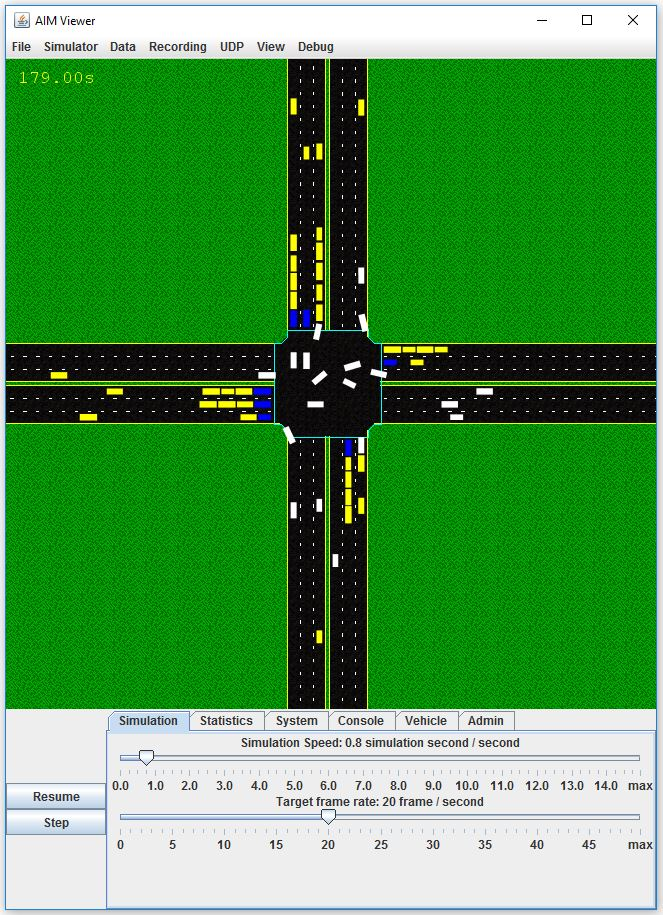
\includegraphics[width=\textwidth]{AIMOriginal.JPG}
\caption{Screenshot of the AIM Simulator}
\end{figure}

A grid-based reservation system works well in high traffic zones like intersections because it forces all vehicles to communicate with a single entity. This achieves a global-view of activity at that junction making it much easier to manage. A V2V solution would require complex communication protocols, possibly with large numbers of vehicles.

However, using a centralised system does create a single point of failure. If the system fails it could lead to collisions in the intersection with the AVs having no way to determine whether it is safe to enter or not. A V2V system would be more fault tolerant, with vehicles being able to navigate their way through a system by themselves.

A centralised system for lane changing was described in a paper by Atagoziyev et al. in 2016 \citep{Atagoziyev2016}. This system uses roadside infrastructure to help groups of vehicles change lanes before they reach a 'critical-position'. These critical-positions could be areas such as motorway exits or intersections.

The vehicles send their position and velocity information to the roadside infrastructure and the system then sends a number of orders to the vehicles such that they safely rearrange themselves into the correct lanes. 

Because the distances involved can be large, particularly at high speeds, the system would struggle to use a reservation tile based system as AIM did, instead it manages the gaps between vehicles to safely relocate vehicles into the correct positions. A more comprehensive overview is given in \ref{subsec:Lane Changing to hit a target lane}.

This system again works very well here because critical points will tend to be high traffic areas so it helps to deal with the issue of large volumes of V2V communications. It also falls into the same pitfall of being a single point of failure. In fact you could argue that for situations such as motorway exits, the consequences of failure are much more severe.

\section{Making lane changing decisions}
\label{sec:Making lane changing decisions}
There are a number of reasons that a driver would want to change lanes. The most obvious being that the overall journey the driver wishes to complete requires the vehicle to move into a different lane. In this case the vehicle \emph{must} change lanes before a 'critical point'. Beyond this point the driver will need to change their planned route, most likely extending their journey time. 

Another reason a driver might change lanes is in order to increase velocity, with the aim of reducing journey time. In general, a driver will aim to change lanes if their average velocity in their current lane is much less than that the velocity it could be achieving in another lane.

\subsection{Lane Changing to hit a target lane}
\label{subsec:Lane Changing to hit a target lane}
In 1986 Gipps' modelled driver behaviour in real world circumstances, characterising the decisions a driver has to make in order to determine whether to change lanes. The paper was designed to be used with the Gipps' 1981 car-following model \citep{Gipps1981}, explained in \ref{sec:Car Following Models}.

The model itself is constructed as a flow chart, in which the decision nodes are the choices a driver must make. 

\todo{Create flowchart figure}

After determining whether a lane change is feasible the model considers whether the driver needs to move into another lane because they are heading towards a critical point.

These decisions are modelled in nodes 3 and 4.

\begin{enumerate}
\item[3] \textit{Driver behaviour close to the intended turn}

If the driver is close to their intended turn then they will always attempt to change into their preferred lane. Only if blocked will they consider moving into another lane. 

'Close' varies depending on regional differences and the level of traffic, but in the model, close is defined as the driver being within a distance equal to ten seconds of travel from the turn at the driver's desired speed.

\item[4] \textit{Urgency of changing lanes}

The urgency of changing lanes increases as the driver gets closer to their turn. The willingness of the driver to brake harder and accept smaller gaps increases as the driver gets closer to their intended turn.

In the implementation, the braking rate a driver is willing to when first becoming close doubles by the time the intended turn is reached. 

\begin{itemize}
\item[$D_n$] is the location of the intended turn
\item[$V_n$] is the desired (or free) speed of the driver
\item[$b_n^*$] is the most severe braking the driver would otherwise be willing to undertake
\end{itemize}

\begin{equation}
b_n = \Biggl[2 - V_n\frac{(D_n - x_n(t))}{10}\Biggr]b_n^*
\end{equation}

\end{enumerate}

This driver decision model is useful, and a good example of a decentralised system. Each driver's decisions are made without a global view of all other drivers. The driver simply adjusts their behaviour as they approach their turn. This provides a fault tolerant solution to the problem, where one vehicle can compensate for the failings of another. However, this does leave the system open to failures due to poor organisation between vehicles. 

Atagoziyev et al. method forces vehicles to work together to manage lane changes before the critical point. The notation for the Atagoziyev model is

\begin{itemize}
\item Vehicles and Points
\begin{itemize}
\item[CP] is the critical point
\item[SV] is the subject vehicle. The vehicle making a lane change.
\item[CL] is the vehicle in front of the SV in the SV's current lane.
\item[TL] is the vehicle in front of the SV in the target lane.
\item[LV] is the lag vehicle behind SV in the target lane.
\end{itemize}
\item Positions
\begin{itemize}
\item[$x$] is the unknown position of SV
\item[$x_l$] is the unknown position of LV
\item[$x_{cl}$] is the trajectory of CL
\item[$x_{tl}$] is the trajectory of TL
\item[$x(t)$] is the position of SV at time $t$
\item[$x_{cl}(t)$] is the position of CL at time $t$
\item[$x_{tl}(t)$] is the position of TL at time $t$
\item[$x_l(t)$] is the position of LV at time $t$
\item[$x_{clb}$] is the CL bound. SV must be located behind this bound during the lane change.
\item[$x_{tlb}$] is the TL bound. SV must be located behind this bound during the lane change.
\item[$x_{lb}$] is the LV bound. SV must be located in front of this bound during the lane change.
\item[$x_{min}(t)$] is the minimum of $x_{tlb}$ and $x_{clb}$ at time $t$
\end{itemize}
\item Times
\begin{itemize}
\item[$t_{end}$] is the available time until the 'string leader' reaches the critical point. The string is the set of cars involved in changing lanes.
\item[$0,t_{end}$] is the time interval available for the lane change manoeuvre.
\item[$\hat{t}$] is the earliest possible time a lane change of SV can be performed.
\item[$\Delta_{LC}$] is the time taken to change lanes.
\item[$W$] is the set of time windows where the leader vehicles enabled a lane change. It is given as 
\begin{equation}
W = {[t_1,t_2]|t_2 \ge t_1 + \Delta_{LC} \land v_{cl}(t) = v_{tl}(t) = v_{nom} \forall t \in [t_1,t_2]}
\end{equation}
\end{itemize}
\item Velocities
\begin{itemize}
\item[$v_{nom}$] is the nominal speed of the vehicles.
\item[$v_{up}$] is faster than average velocity.
\item[$v_{dn}$] is slow than average velocity.
\item[$v_{cl}$] is the CL velocity.
\item[$v_{tl}$] is the TL velocity.
\item[$v_{min}(t)$] is the minimum of $v_{tlb}$ and $v_{clb}$ at time $t$
\end{itemize}
\end{itemize}

The Atagoziyev model performs a number of lane changes in order to rearrange the vehicles into the right lanes. To do this it loops through all of the vehicles that aren't in the right lane.

\todo{Explain all of the Atagoziyev model? It seems excessive.}

\subsection{Lane Changing to improve overall velocity}
\label{subsec:Lane Changing to improve overall velocity}
Gipps' driver decisions model also considered situations where the driver does not have to be in any particular lane. The model considers the effects of transit lanes, heavy vehicles and the effect of the preceding vehicle on the driver's vehicle. These are shown in nodes 5 to 7 and 9 to 11.

\begin{enumerate}
\item[5] \textit{Transit vehicles and lanes}
Transit lanes are lanes dedicated solely for public transport and other high occupancy vehicles. These include vehicles such as buses, taxis and carpool cars. These vehicles are known in the model as 'transit vehicles'.
\item[6] \textit{Entry of nontransit vehicles into transit lanes}
If there is an obstruction in the present lane, it is often considered to be a valid reason for a non-transit vehicle to enter a transit lane. 
\item[7] \textit{Departure of nontransit vehicles from a transit lane}
Once the obstruction has been cleared, nontransit vehicle must move back into a valid lane. This forced departure does not affect vehicles that are close to their intended turn.
\item[9] \textit{Relative advantages of present and target lanes}
If the driver has not yet been forced to change lanes by any other factors, then they can look at the relative advantages of the present and target lanes, considering obstructions and then determining which lanes obstructions will have the least effect on their safe speed.
\item[10] \textit{The effect of heavy vehicles} 
If obstructions are level with each other or beyond the range a driver considers, then the driver considers the next heavy vehicle in each lane, as if it were the leading vehicle in an ordinary car following situation. The driver then selects the lane which will give them the higher speed.
\item[11] \textit{The effect of the preceding vehicle}
If there are then no heavy vehicles, the driver considers the speed possible in each lane and then changes if they gain a 'sufficient' speed advantage. This is again, subjective, depending on the present lane, target lane and the type of vehicle.
\end{enumerate}

In areas where traffic is flowing quickly and there aren't a large number of vehicles to organise around, decentralised models like this work very well. Vehicles can act independently of each other fairly easily. However, Gipps' model is based on human interaction and does not consider the global effect of a lane change. The work by Kesting et al. in 2007 \citep{Kesting2007} produces a decentralised model for lane changes which also considers the effect of your lane change on other vehicles. This can help to reduce the 'phantom intersection' effect and improve overall traffic flow.

\todo{Explain what Kesting did and compare it to Gipps' model.}